\chapter{Strumenti e tecnologie}
\label{cap:strumenti-tecnologie}

\intro{L'obiettivo principale di questo capitolo è l'illustrazione delle tecnologiene degli strumenti ausiliari utilizzati per raggiungere lo scopo finale del progetto}\\

\section{Strumenti}
\label{sec:strumenti}
Gli strumenti di supporto adoperati per il progetto sono elencati nella lista seguente.

\subsection{Visual Studio Code}
Visual Studio Code (Fig.~\ref{fig:logo-vscode}): è un ambiente di sviluppo integrato, disponibile per Linux, macOS e Windows. 
È un'applicazione che supporta la maggior parte dei linguaggi di programmazione ed è quindi molto vantaggiosa per lavorare ad un progetto multi-linguaggio senza dover cambiare ambiente.
Un'altra delle funzionalità principali è la fornitura di numerose estensioni che semplificano il processo di scrittura e verifica del codice.

\begin{figure}[!h] 
    \centering 
    
\includegraphics[width=0.4\columnwidth]{tecnologie/visual-studio-logo.png} 
    \caption{Logo di Visual Studio Code}
    \label{fig:logo-vscode}
  \end{figure}

\newpage

\subsection{PhpMyAdmin}
PhpMyAdmin (Fig.~\ref{fig:logo-phpmyadmin}): è una web-app scritta utilizzando il linguaggio di programmazione PHP, che offre la capacità di gestione di un database MySQL attraverso un browser qualsiasi. Consente la creazione di tabelle, l'inserimento, la modifica e l'interrogazione dei dati.
Fornisce un'interfaccia grafica per la visione d'insieme e per le operazioni amministrative.

\begin{figure}[!h] 
      \centering 
      
\includegraphics[width=0.4\columnwidth]{tecnologie/phpmyadmin-logo.png} 
      \caption{Logo di phpMyAdmin}
    \label{fig:logo-phpmyadmin}
  \end{figure}

\subsection{remoteripple}
Remote Ripple (Fig.~\ref{fig:logo-remoteripple}): è un software per l'accesso remoto, che viene utilizzato dallo studente per avviare i programmi presenti nel server aziendale.
    
\begin{figure}[!h] 
    \centering 
    
\includegraphics[width=0.3\columnwidth]{tecnologie/remote-ripple-logo.png} 
    \caption{Logo di Remote Ripple}
    \label{fig:logo-remoteripple}
  \end{figure}


\newpage

\section{Tecnologie}
\label{sec:tecnologie-strumenti}

Nelle sezioni seguenti viene data una spiegazione di tutte le tecnologie utilizzate.

\subsection{Python}

\subsubsection{Versione: 3.9.0}
Python (Fig.~\ref{fig:logo-python}) è un linguaggio di programmazione ampiamente utilizzato in settori come il data mining e l'intelligenza artificiale. 
Offre solide basi per l'integrazione con disparati linguaggi, ma il vantaggio più di risalto è la presenza di numerose librerie che aiutano lo sviluppatore a velocizzare il processo di codifica; in particolare sono state utilizzate le seguenti librerie:

\subsubsection{\label{tec:tensorflow}Tensorflow-gpu 2.10.1}

TensorFlow è una framework utilizzato per il machine-learning, su di esso si basa tutta la struttura del progetto.\\
L'unità di base del framework è il tensore, ossia un vettore di n dimensioni, tutte le operazioni possibili vengono eseguite su elementi appartenenti a questo tipo.
Inoltre contiene modelli pre-addestrati molto utili per eseguire determinate operazioni in maniera più rapida. 
Viene utilizzata la versione 2.10 perché è l'ultima ad avere il supporto per GPU su sistema operativo Windows.

\subsubsection{Keras 2.10.0}
Keras è un API sviluppata per rendere la codifica di IA più semplice per la comprensione umana. 
Minimizza le azioni richieste all'utente per i casi d'uso più comuni, rendendo l'utilizzo di framework come JAX, TensorFlow e PyTorch più user-friendly.

\subsubsection{Scikit-Learn 1.5.2}
Scikit-learn è una libreria che offre semplici tool utili per la classificazione, la regressione, il clustering, eccetera.

\subsubsection{Matplotlib 3.9.2}
Matplotlib è una libreria che viene utilizzata per la stampa dei grafici ottenuti durante le varie compilazioni. 

\subsubsection{Numpy 1.26.4}
Numpy è il pacchetto che si occupa della gestione di array multi dimensionali fornendo anche un'ampia gamma di funzioni matematiche da applicare agli stessi.

\subsubsection{OpenCV-python 4.10.0}
OpenCV è una libreria utilizzata per sviluppare applicazioni di tipo computer vision. Nell'ambito del progetto il suo scopo primario è l'elaborazione delle immagini per adattarle all'utilizzo da parte delle IA. 

\subsubsection{Pyppeteer 2.0.0}
Pyppeteer è una libreria di automazione per browser basati su chromium.

\begin{figure}[!h] 
  \centering 
  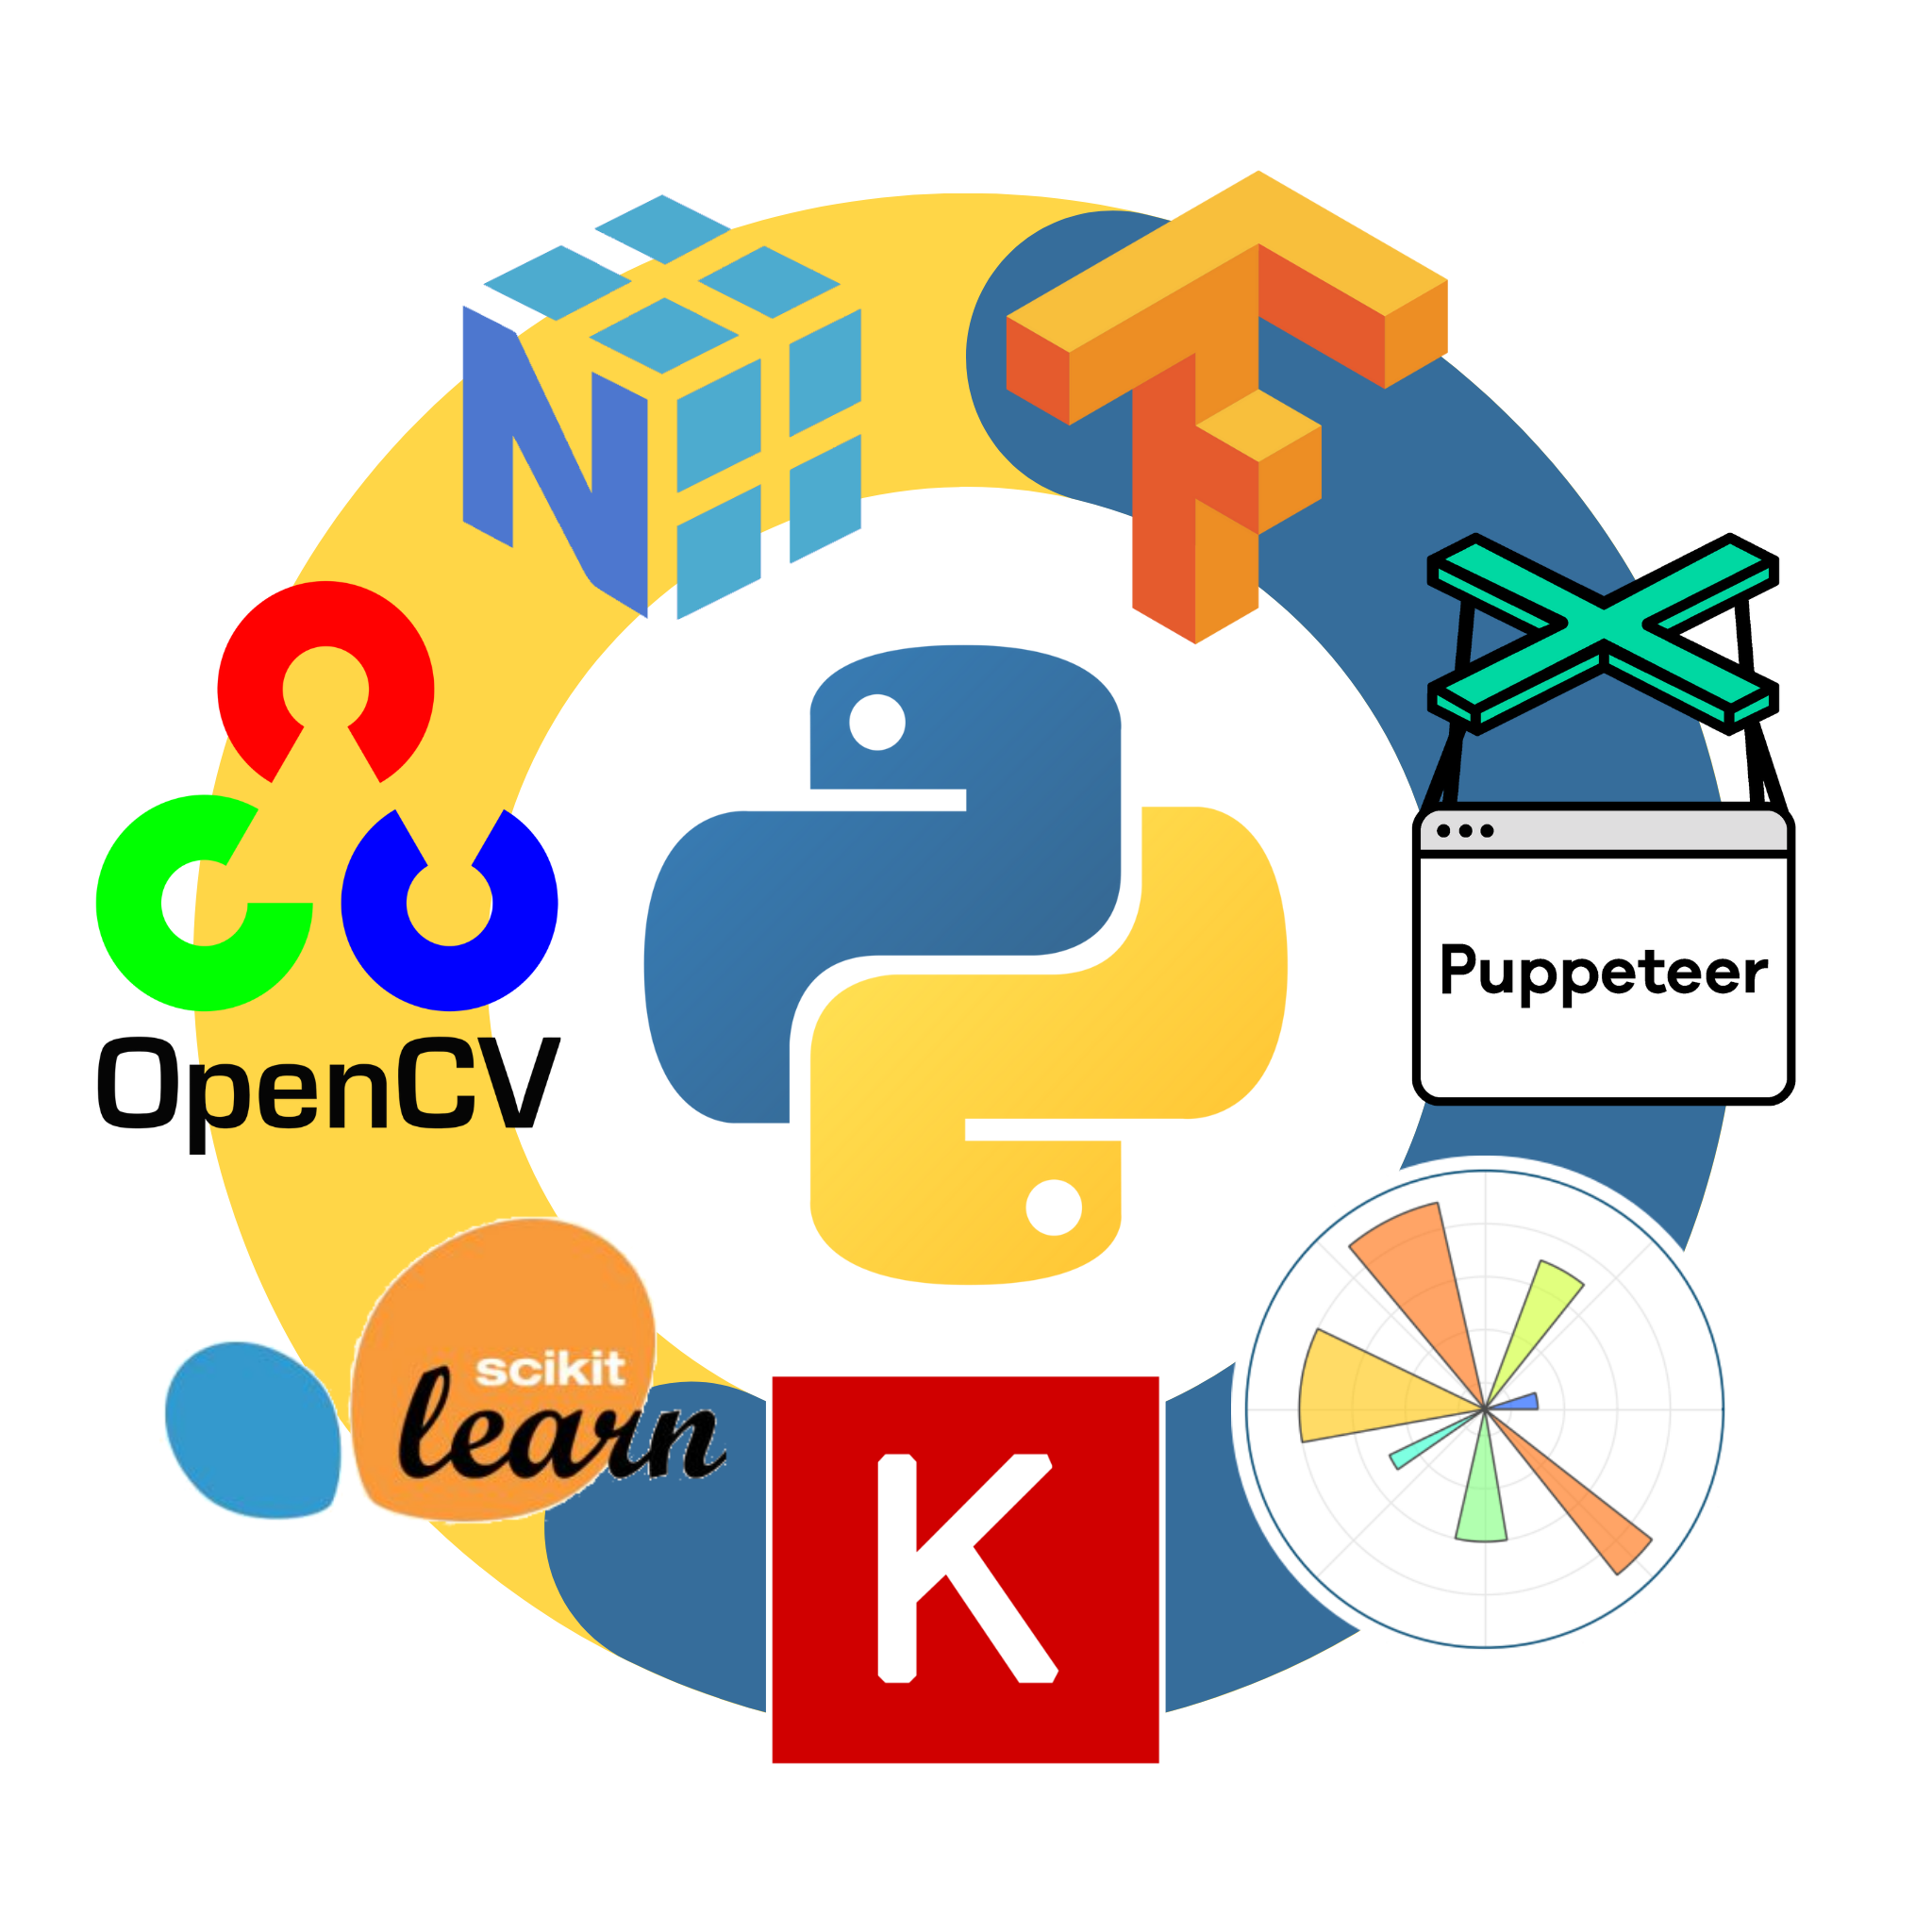
\includegraphics[width=0.8\columnwidth]{tecnologie/python-librerie.png} 
  \caption{Python e librerie utilizzate}
  \label{fig:logo-python}
\end{figure}


\subsection{\label{tec:cuda}CUDA}
\subsubsection{Versione: 11.2}
CUDA (Fig.~\ref{fig:logo-cuda}) è un toolkit che fornisce un ambiente di sviluppo in grado di creare applicazioni che sfruttino a pieno le GPU di NVIDIA.
Nel caso di studio CUDA è un elemento portante in quanto fornisce a Python e alle sue librerie la capacità di eseguire calcoli in maniera più rapida utilizzando la GPU.
La GPU hanno un'architettura diversa rispetto alle CPU che consente loro di eseguire parallelamente più operazioni, per questo sono molto portate per l'addestramento delle IA.
La versione 11.2 viene utilizzata perché è l'unica compatibile con \nameref{tec:tensorflow}.

\begin{figure}[!h] 
  \centering 
  
\includegraphics[width=0.5\columnwidth]{tecnologie/cuda-logo.png} 
  \caption{Logo di CUDA}
  \label{fig:logo-cuda}
\end{figure}

\newpage

\subsection{\label{tec:docker}Docker}
\subsubsection{Versione: 27.2.0}
Docker (Fig.~\ref{fig:logo-docker}) è un sistema che consente di semplificare lo sviluppo delle applicazioni fornendo un ambiente isolato e facilmente riproducibile. Tale ambiente viene definito come container, al suo interno vengono eseguite le immagini di tutti i componenti necessari per il funzionamento dell'applicativo; senza che sia necessario installarli sulla propria macchina.

\begin{figure}[!h] 
  \centering 
  
\includegraphics[width=0.5\columnwidth]{tecnologie/docker-logo.png} 
  \caption{Logo di Docker}
  \label{fig:logo-docker}
\end{figure}


\subsection{\label{tec:ddev}DDEV}
\subsubsection{Versione: 1.23.2}
DDEV (Fig.~\ref{fig:logo-ddev}) è un tool per velocizzare il lancio di ambienti di sviluppo web in locale; consente di utilizzare il workflow di \nameref{tec:docker} in maniera più rapida.

\begin{figure}[!h] 
  \centering 
  
\includegraphics[width=0.25\columnwidth]{tecnologie/ddev-logo.png} 
  \caption{Logo di DDEV}
  \label{fig:logo-ddev}
\end{figure}

\newpage

\subsection{\label{tec:wsl}WSL}
\subsubsection{Versione: 2.3.24.0}
WSL (Fig.~\ref{fig:logo-wsl}) è un sottosistema che viene utilizzato per eseguire applicazioni create per il sistema operativo Linux su Windows.

\begin{figure}[!h] 
  \centering 
  
\includegraphics[width=0.3\columnwidth]{tecnologie/wsl-logo.png} 
  \caption{Logo di WSL}
  \label{fig:logo-wsl}
\end{figure}

\subsection{\label{tec:Laravel}Laravel}
\subsubsection{Versione: 11.29.0}
Laravel (Fig.~\ref{fig:logo-laravel}) è un framework ideato per la creazione di web-application scritto in PHP.
Tra i suoi vantaggi abbiamo la semplicità della sintassi, il supporto continuo della community e la presenza di numerosi tutorial che è fondamentale per fornire a sviluppatori alle prime armi l'aiuto necessario.
Laravel si basa sul pattern architetturale MVC (Model View Controller):
\begin{itemize}
  \item Model: accede ai dati contenuti nell'applicativo.
  \item View: mostra i dati contenuti nel model e gestisce le interazioni con gli utenti.  
  \item Controller: riceve le operazioni degli utenti e modifica di conseguenza i dati contenuti nel model e la visualizzazione mostrata dalla view.
\end{itemize}

\begin{figure}[!h] 
  \centering 
  
\includegraphics[width=0.3\columnwidth]{tecnologie/logo-laravel.png} 
  \caption{Logo di Laravel}
  \label{fig:logo-laravel}
\end{figure}

\newpage 

\subsection{\label{tec:Filament}Filament}
\subsubsection{Versione: 3.2.121}
Filament (Fig.~\ref{fig:logo-filament}) è un framework basato su \nameref{tec:Laravel} che fornisce la possibilità di generare componenti per l'interfaccia grafica (Fig.~\ref{fig:gui-filament}) in maniera rapida.

\begin{figure}[!h] 
  \centering 
  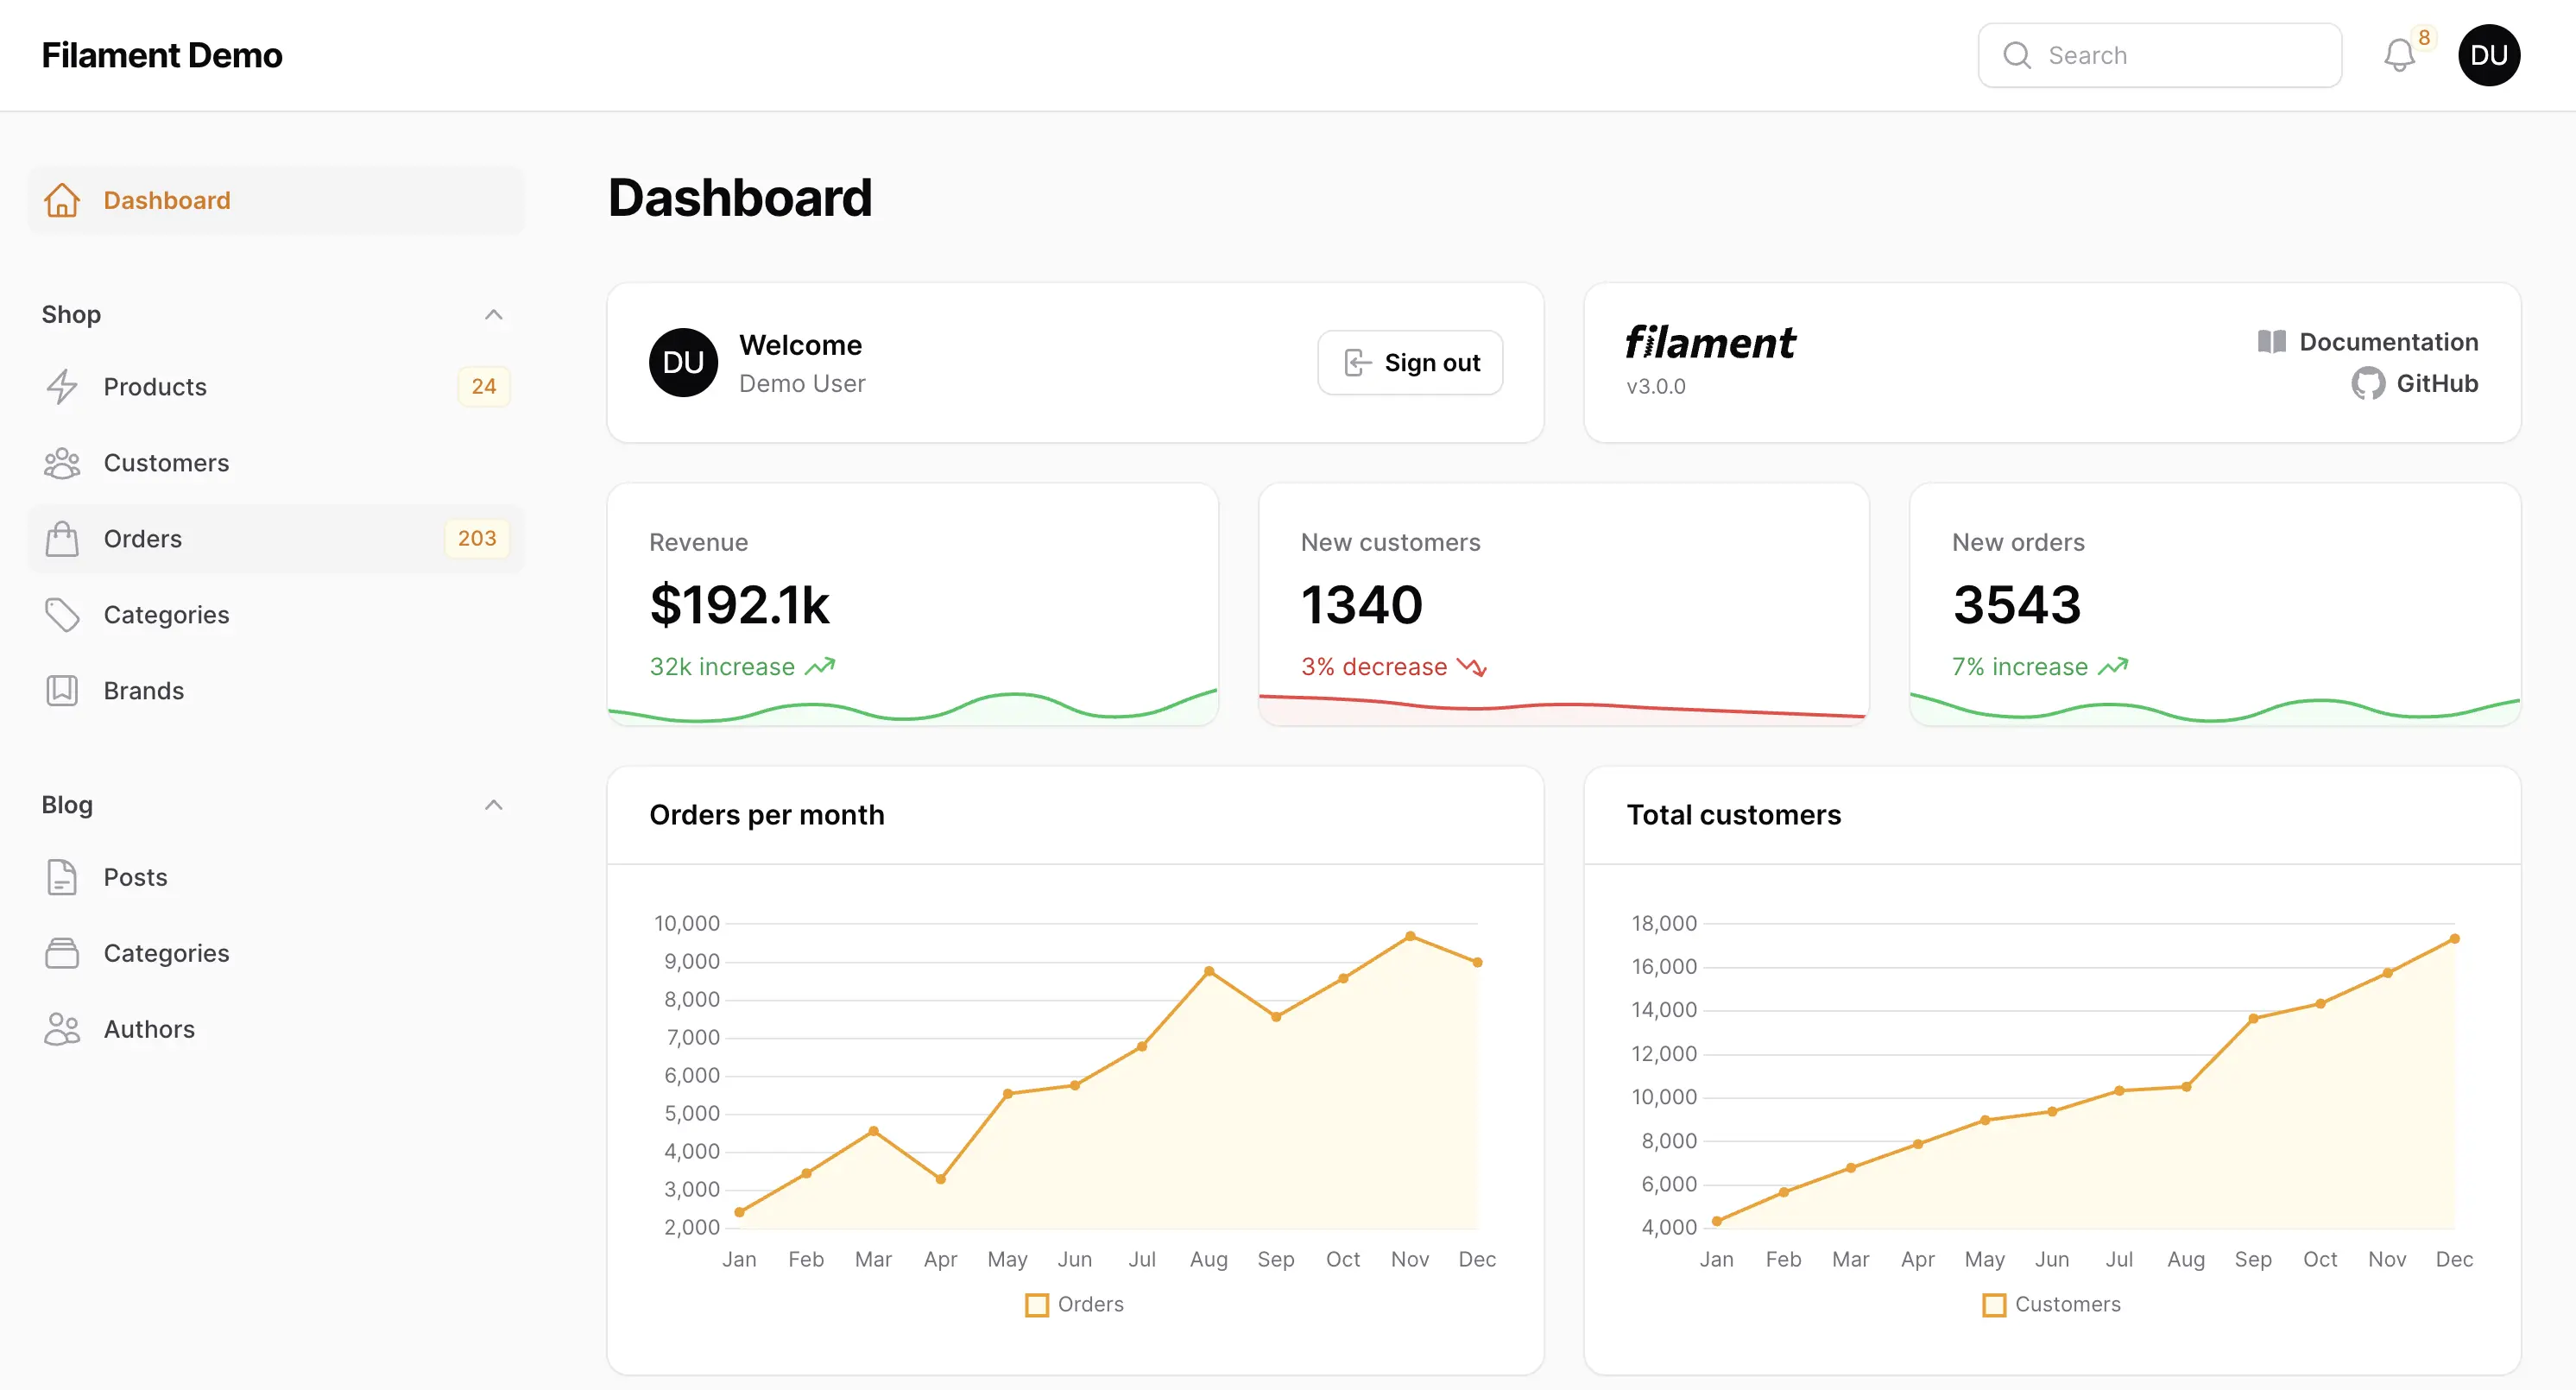
\includegraphics[width=0.8\columnwidth]{tecnologie/filament-demo.png} 
  \caption{Esempio di interfaccia grafica creata in Filament}
  \label{fig:gui-filament}
\end{figure}

\begin{figure}[!h] 
  \centering 
  
\includegraphics[width=0.3\columnwidth]{tecnologie/filament-logo.png} 
  \caption{Logo di Filament}
  \label{fig:logo-filament}
\end{figure}

\newpage

\subsection{\label{tec:mysql}MySQL}
\subsubsection{Versione: 8.0.36}
MySQL (Fig.~\ref{fig:logo-mysql}) è un database relazionale open-source.

\begin{figure}[!h] 
  \centering 
  
\includegraphics[width=0.3\columnwidth]{tecnologie/mysql-logo.png} 
  \caption{Logo di MySQL}
  \label{fig:logo-mysql}
\end{figure}

%AGGIUNGERE DA QUALCHE PARTE LE DIPENDENZE TRA LIBRERIE E VERSIONI

